\documentclass[../../main]{subfiles}

\renewcommand\thesection{\arabic{section}}


\begin{document}

\section{Thermal Monitoring} \label{sec:}

For effectively controlling the indoor temperature of the Incubator, a \emph{paired} temperature
sensor would be essential. One will monitor the \emph{outdoor} temperature, as the other monitors
the \emph{indoor} temperature. From the output of each of these sensors, a \emph{relative} temperature
can be estimated and the \emph{heating and cooling system} can be tweaked accordingly.

\subsection{DHT22}

\begin{center}
    {\begin{minipage} [c] {0.55\textwidth}

        First of all we need a \emph{sensor} to measure the temperature reliably.
        \emph{DHT22}, a sensor which can measure both the \emph{relative humidity}\footnote{EMCU will monitor
        and control \emph{air moisture} too.} and \emph{temperature} would be ideal choice for our scenario.
        Another advantage of \emph{DHT22} is that the communication is done via a single pin.
        Please refer the figure \ref{fig:dht22PinImage} for a quick glance at the sensor.

        General and temperature specification:

        \begin{itemize}
            \item \textbf{Operating voltage:} $3.3\si{V}$ to $6\si{V}$.
            \item \textbf{Sensing period:} $2$ seconds.
            \item \textbf{Temperature range:} $-40^\circ$C to $80^\circ$C, with $\pm 0.5^\circ$C tolerance.
            \item \textbf{Temperature resolution:} $0.1^\circ$C.
        \end{itemize}

    \end{minipage}
    \hfill
    \begin{minipage} [c] {0.35\textwidth}
        \centering
        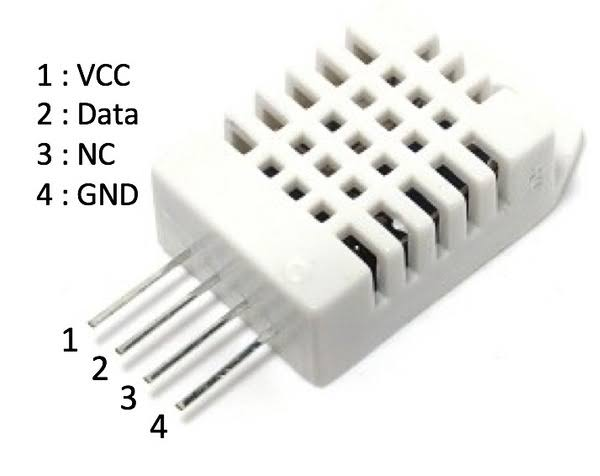
\includegraphics [
            max width = \IGXMaxWidth,
            max height = \IGXMaxHeight,
            \IGXDefaultOptionalArgs,
        ] {pics/dht22.png}
        \captionof{figure} {
            Pinout of \emph{DHT22} sensor.
            \label{fig:dht22PinImage}
        }
    \end{minipage}\hfill}
\end{center}

Also refer figure \ref{fig:absThermalSensorSystem} for the interfacing of \emph{DHT22} sensors
to the rest of the EMCU.

\begin{figure}
    \centering
    \includegraphics [
        max width = \IGXMaxWidth,
        max height = \IGXMaxHeight,
        \IGXDefaultOptionalArgs,
    ] {tikzpics/endAbsThermalSensorSystem.pdf}
    \captionof{figure} {Interfacing of \emph{DHT22} through multiplexer.}
    \label{fig:absThermalSensorSystem}
\end{figure}

\alertWarning{
    The \emph{BUF} and \emph{0/1} blocks of figure \ref{fig:absThermalSensorSystem} are part of
    the \emph{auxiliary system} that is not implemented\footnote{there will be a circuit that
    helps to enable and disable different systems.} yet. Right now the power pins of the sensors
    are tied directly to $3.3\si{V}$.
}

\alertNote{
    Data pins of \emph{DHT22} sensors are connected to the \texttt{C7} and \texttt{C8} pins of
    $32$ bit multiplexer.
}

\end{document}
